\TOWRITE{NT/...}{Finalise}
\TOWRITE{ALL}{Proofread concept and approach pass 2}

\subsection{Concept and Approach}\label{sec:concept}
\eucommentary{5-8 pages}
\eucommentary{
-- Describe and explain the overall concept underpinning the project.
Describe the main ideas, models or assumptions involved. Identify
any trans-disciplinary considerations;
-- Describe and explain the overall approach and methodology, distinguishing, as
appropriate, activities indicated in the relevant section of the work programme, e.g.
Networking Activities, Service Activities and Joint Research Activities, as detailed in
the Part E of the Specific features for Research Infrastructures of the Horizon 2020
European Research Infrastructures (including e-Infrastructures) Work Programme 2014-
2015;\\
-- Describe how the Networking Activities will foster a culture of co-operation between the
participants and other relevant stakeholders.\\
-- Describe how the Service activities will offer access to state-of-the-art infrastructures,
high quality services, and will enable users to conduct excellent research.\\
-- Describe how the Joint Research Activities will contribute to quantitative and qualitative
improvements of the services provided by the infrastructures.\\
-- As per Part E of the Work Programme, where relevant, describe how the project will
share and use existing basic operations services (e.g. authorisation and accounting
systems, service registry, etc.) with other e-infrastructure providers and justify why such
services should be (re)developed if they already exist in other e-infrastructures. Describe
how the developed services will be discoverable on-line.\\
-- Where relevant, describe how sex and/or gender analysis is taken into account in the
project's content.}


\begin{figure}[ht]\centering
  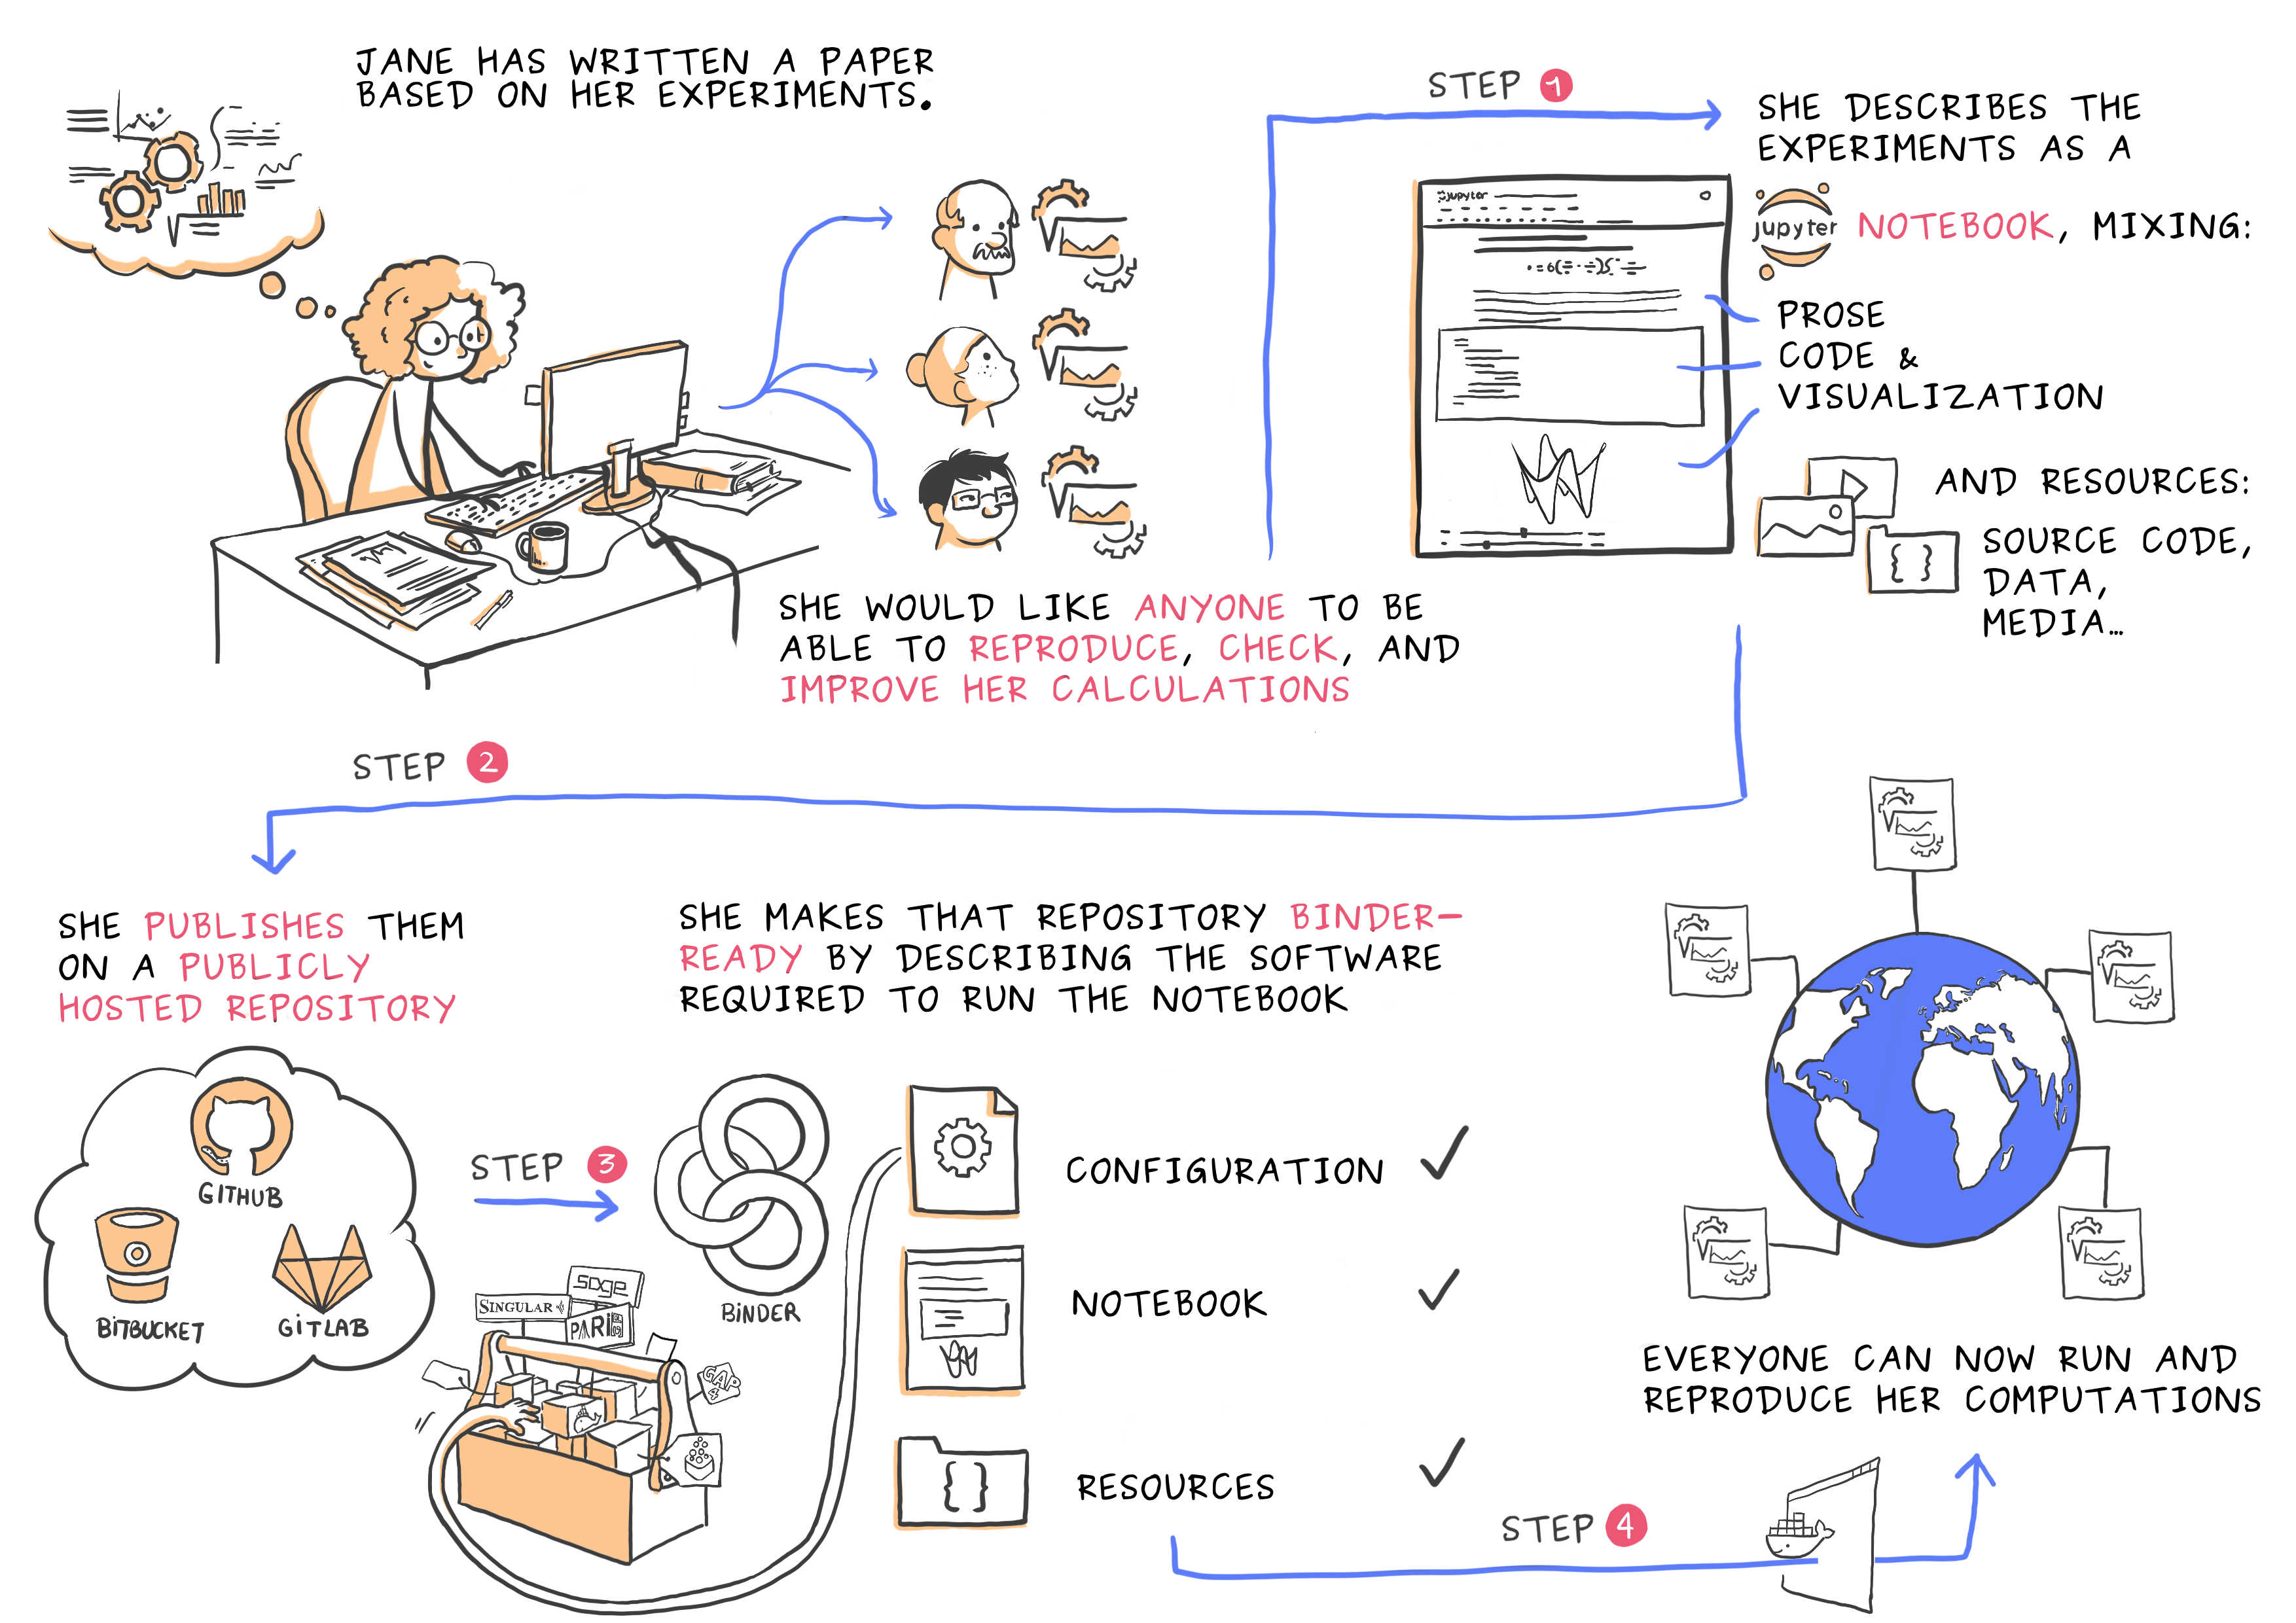
\includegraphics[width=0.9\textwidth]{use-cases-binder-logbook-solution.png}
  \caption{A typical use case for Jupyter notebooks in research.
            Image by Juliette Belin for the OpenDreamKit project, used under
            CC-BY-SA.}\label{fig:use-cases-binder}
\end{figure}


Open Science is the principle that science, in order to be most
impactful and socially responsible, should be done publicly, with as
much of the scientific process and products accessible, reviewable,
and reusable by as many members of the global community as possible.
In the modern age of computational science, almost all academic
fields, from humanities to social sciences to biology and astronomy
are faced with exciting opportunities for Open Science.  As more and
more research takes the form of code and/or data, the opportunity to
share, reproduce, and reuse scientific work is greater than ever, even
enabling new forms of interdisciplinary collaboration.

At the same time as we share in these exciting opportunities, there
are corresponding challenges, technical and social, to making Open
Science a practical reality.  We face big questions: If a researcher
has code and/or data to publicise, how is that best done?  How do
researchers learn best Open Science practices in their field?  How do
previously disconnected fields benefit from each other's work as the
same computational challenges are faced again and again by different
communities?

These are the questions that guide \TheProject.
With so much research being done that wants to be Open,
how can we make Open Science

\begin{enumerate}
    \item as easy as possible to share?
    \item as useful as possible to other researchers and the public?
\end{enumerate}

\noindent Our plan for improving access and effectiveness of Open Science can be summarised as:

\begin{enumerate}
\item improve and maintain common software infrastructure used for
  Open Science
\item develop the Jupyter ecosystem to improve capabilities better
  serve Open Science
\item guide, validate, and demonstrate our developments through
  collaboration with a wide variety of application domains
\item enable students and researchers to perform Open Science through
  training and education, and improving inclusiveness by focusing
  these on under-served and under-represented communities.
\item operate services to facilitate Open Science collaborations with
  Jupyter software
\end{enumerate}

\textbf{Why Jupyter?}

\TheProject has chosen to centre its efforts on the Jupyter software
ecosystem.  The Jupyter notebook and Jupyter ecosystem is of
increasing importance in computational science and data science, in
academia, industry and services. In addition to supporting high
productivity of researchers, they have great potential to push open
science forward: the notebook provides a complete description of a
computational and data science study, and the notebook can -- in
principle -- be turned into a publication, or can be used to provide
the required computation for a part of a publication, such as a
figure. In this way, the notebook enables reproducibility of complex
tasks with hardly any additional effort on the user side (if used
appropriately). The Binder project allows to execute such notebooks in
tailored computational environments; an aspect of reproducibility that
is not widely supported yet. Furthermore, for users wanting to connect
to a local Jupyter notebook server on their machine, or to connect to
a server somewhere else on the Internet, the users only need a
webbrowser to display the notebook locally. Because of these
characteristics, the Notebook is already planned to become an
important service on the European Open Science Cloud (EOSC), for
example through the EOSC-04 funded PaNOSC project.

\TOWRITE{}{short definition of Jupyter components, mixing code \& prose, etc. }

Because the Jupyter notebook is a web-based application, it can be
deployed at computational facilities or in the cloud, and can function
as the basis for services exposing computational resources of all
kinds to researchers and the public.  Because Jupyter is
\textit{interactive}, it enables making scientific results and
communications more interactive than static publications.  The
audience can follow their own initiative and ask their own questions
of published data without needing support from the publishing author,
greatly facilitating the \textit{practicality} of Open Science.

\textbf{Jupyter is generic} \TheProject chose Jupyter because it is
Generic.  Jupyter makes no domain-specific or even language-specific
assumptions.  Any application where mixing description, code, and
results is valuable can make use of Jupyter.  This broad applicability
makes investment in the Jupyter ecosystem extremely effective, because
improvements to Jupyter can serve many communities simultaneously.

Jupyter is built from a collection of standard protocols and file
formats.  Jupyter is not just a single, monolithic collection of
software, but a description of how such software can be built.  The
result is the ability for a variety of communities and applications to
use pieces of Jupyter for their purposes, and/or reimplement pieces to
meet their needs.

For example:

\begin{enumerate}
\item The notebook file format is a well-specified JSON document,
  which can be interpreted by many systems.  This has facilitated the
  development of different services rendering notebooks, e.g. the code
  hosting website GitHub, which renders notebooks for easy viewing by
  anyone, without Jupyter software.
\item the Jupyter protocol describes how execution is performed, which
  has enabled the development of over one hundred kernel
  implementations in dozens of languages.
\item output in the Jupyter protocol uses web-standard MIME types,
  enabling any possible format to be an output in a Jupyter notebook.
\item the JupyterLab extension system provides a system for building
  applications from Jupyter components and others
\item the Jupyter Widgets provide a system for customizing and
  extending interactivity in Jupyter-based environments
\end{enumerate}

The popularity of Jupyter, with millions of users and hundreds of open
source contributors, indicates the value and impact of this approach.

\textbf{How do we improve Jupyter?}

The benefits of focusing our work on a mature system like Jupyter are

\begin{itemize}
\item vibrant community ensures health and sustainability
\item large existing user base maximises impact of contributions
\item mature software ecosystem maintains quality software through
  industry standards such as version control, tests, continuous
  integration, stable release cycles, roadmaps, and user support
\end{itemize}

The Jupyter community aims to be inclusive, and \TheProject will
continue this effort.  Jupyter is inclusive across a number of axes.
By being applicable across numerous domains, Jupyter and \TheProject
encourage participation from individuals of various interests and
backgrounds, and has taken action to improve diversity in the project
by participating in "Outreachy," a program of paid internships for
individuals from groups that face under-representation, systemic bias,
or discrimination.  Jupyter has also operated workshops focused on
training contributors from under-represented groups.  In being free,
public, open source software, Jupyter and \TheProject are accessible
to as many individuals as possible, and invites users and contributors
beyond origin, nationality, beliefs, orientation.  One area where
Jupyter has lacked in this regard is in the User Interface
accessibility, and we will help improve this in
\taskref{jupyter-core}{accessibility}.  Additionally, the project will
focus some of its workshops in \taskref{education}{workshops} on
under-represented communities.




\begin{verbatim}
Outline notes:

* Carry on with specified protocols and formats so that components can be replaced, combined etc.
* Avoid lock-in to specific technologies (for example JupyterHub not limited to AWS but cloud-provide agnostic way) – thus independent from dominating commercial cloud services provider
* Integrating user input in multiple ways
   * User input at JupyterCon: beginners and experience users to try new version of UI; sessions where recorded and used to improve software (“usability testing”)
   * Co-design: developed by scientists for scientists, but professional software engineers and UX designers involved in the design of the software; [deliberate effort because Jupyter is a tool to teach beginners and specialists]
   * UI is at level of polish that is rarely met in non-commercial applications
\end{verbatim}
